\begin{Figure}
\SECTION{2.1 Modelling Memory}
\begin{tikzpicture}[
    spy using outlines={circle
        , magnification=10, connect spies
    }
    ]
    \centering
    \node [] (image) at (0,-1) {
        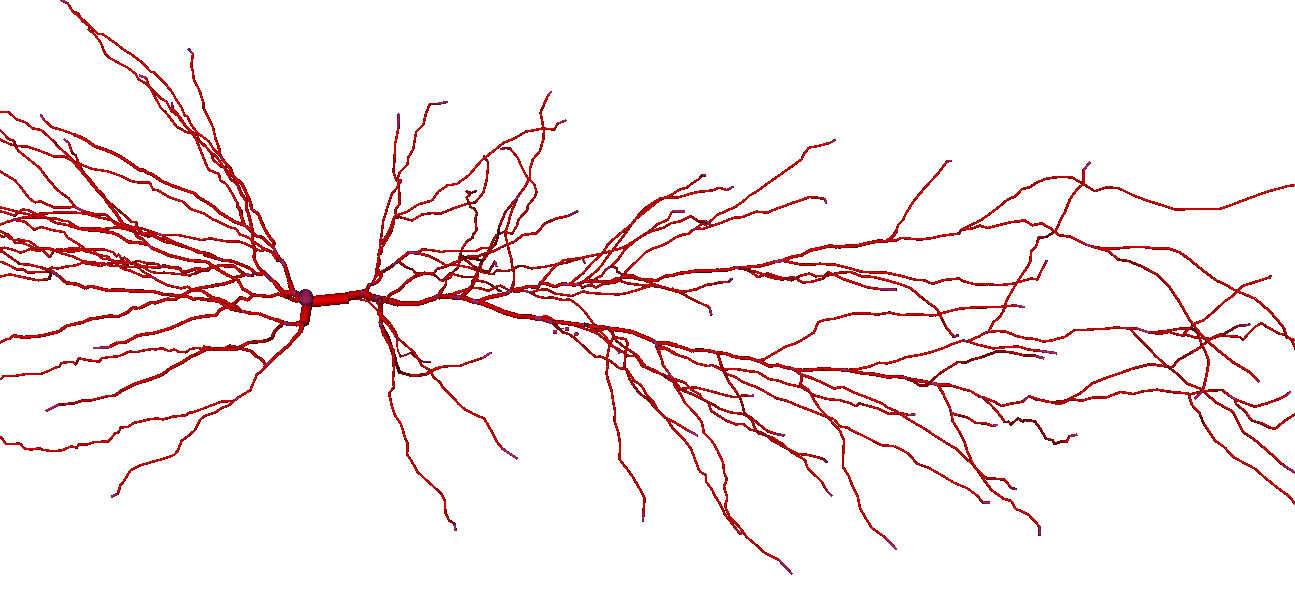
\includegraphics[scale=0.2,angle=-30]{./images/ca1_neuron.png}
    };

    \foreach \i in {-3,...,3}
    \foreach \j in {-3,...,3}
    {
        \node[fill=blue,opacity=0.3,thin,inner sep=0pt, minimum size=3mm,circle] (n\i\j) at (\i, \j) {};
    };

    \spy[blue, size=3cm] on (1.65, -1.5) in node[left] at (7,3);
    \node[below=4cm,text width=0.3\textwidth] {\CAPTION{A single detailed neuron is
            embedded in a network of simple cells}};

    %% Cool. Now create a 3d compartment model here.
    \begin{scope}[xshift=11cm, yshift=3cm
        , compartment/.style={cylinder
            , draw
            , cylinder uses custom fill
            , cylinder end fill = red!35
            , cylinder body fill = red!40
            , inner sep = 3mm
            , minimum height = 1cm
            , minimum width = 1cm 
        }
        , spine/.style={cylinder 
            , fill = blue!20
            , inner sep=1mm
            , minimum height=1mm
            , minimum width=3mm
        }
        , branch/.style={cylinder
            , draw
            , cylinder uses custom fill
            , cylinder end fill = red!35
            , cylinder body fill = red!40
            , minimum height = 1.5cm
            , minimum width = 0.5cm
            , inner sep = 1mm
        }
        ]

        \node[compartment] (c1) {};
        \node[compartment] (c2) at (c1.east) {};
        \node[compartment] (c3) at (c2.east) {};

        \node[branch,rotate=45] (b1) at ([xshift=4mm,yshift=2mm]c3.before top) {};
        \node[branch,rotate=-45] (b2) at ([xshift=1mm, yshift=-7mm]c3.base east) {};

        % Spines
        \node[spine, inner sep=1mm, rotate=135] (s11) at (b1.north east) {};
        \node[spine, inner sep=1mm, rotate=135] (s12) at ([xshift=3mm]b1.south east) {};

        \node[spine, inner sep=1mm, rotate=45] (s21) at (b2.north east) {};
        \node[spine, inner sep=1mm, rotate=45] (s22) at ([xshift=-3mm]b2.south east) {};

    \end{scope}

    %% Scope to draw chemisty 
    \begin{scope}

        \node[] (chemical) at ([yshift=-6cm]c2.south) {
            \includegraphics[width=0.35\textwidth, trim=5mm 5mm 5mm 5mm, clip]{./images/chemical_reactions.png}
        };

        %%  
        \node [above] (chemicallabel) at ([yshift=-2cm]c1.south) {\LARGE{
                Chemical models}};

        \draw[o-o] (c1.center) to [bend right] (chemicallabel.center);

        %% Add transportation model.
        \node[] (transport) at ([xshift=7cm,yshift=-3cm]s12.north) {
            \includegraphics[width=0.3\textwidth]{./images/transport_mechanism.png}
        };

        \node[] (tlabel) at ([xshift=0.5cm, yshift=0cm]transport.north) {\LARGE{Trafficking
                models}};

        \draw[o-o] (s21.center) to [bend left] (tlabel) ;

    \end{scope}
\end{tikzpicture}


\vspace{1cm}
\begin{tikzpicture}
    \node[] (label) at ([xshift=-20cm]tlabel) {
        \CAPTION{\hspace{12cm} Neighbouring spines are modified differently}
    };
\end{tikzpicture}

%% memory results by upi
\begin{tikzpicture}
    \node[] (resultb) {
        \includegraphics[width=0.5\textwidth]{./images/spike_raster.png}
    };
\end{tikzpicture} \hfill %
\begin{tikzpicture}
    \node[] (resultA) {
        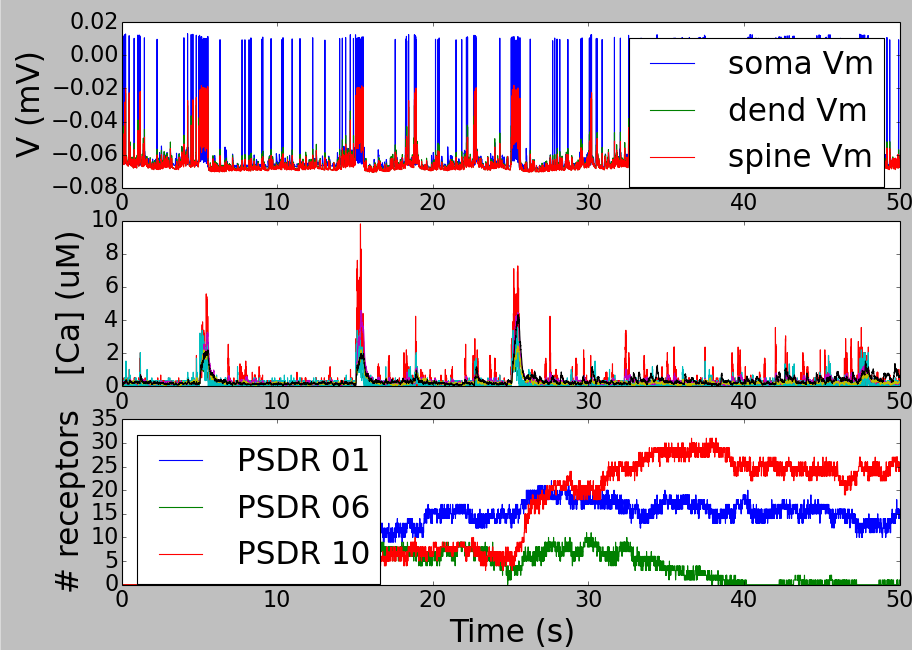
\includegraphics[width=0.5\textwidth]{./images/timeseries.png}
    };
\end{tikzpicture}

\SECTION{2.2 Modelling Olfactory Bulb}
\centering
\begin{tikzpicture}
    \node[] (aditya) {
        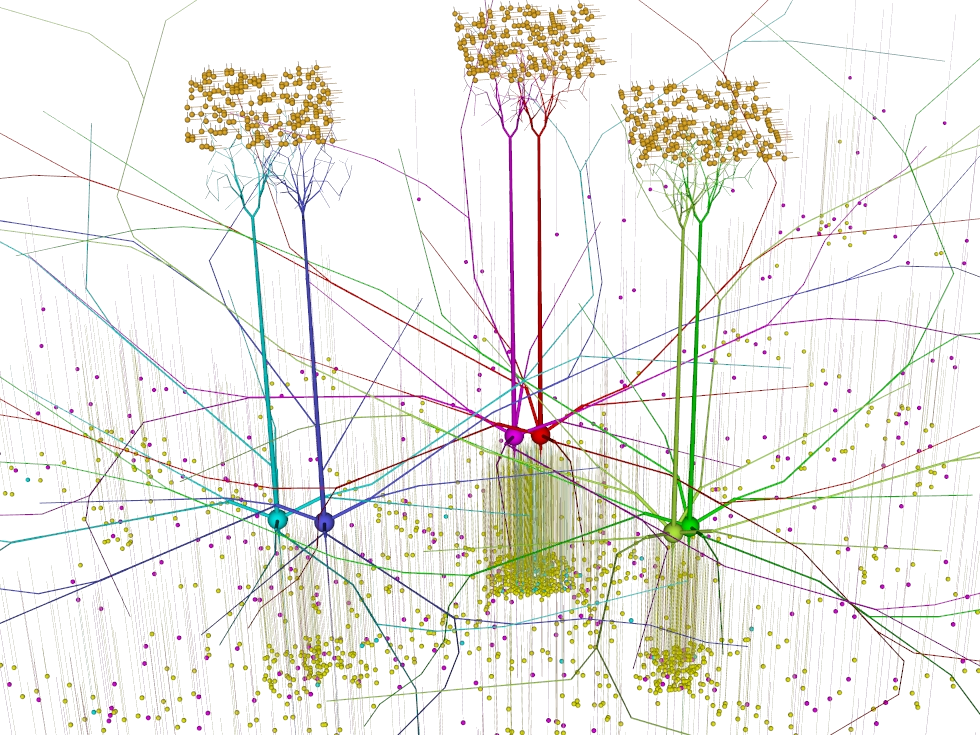
\includegraphics[width=\textwidth]{./images/fullmodel_moogli.png}
    };
\end{tikzpicture}
\vspace{1cm}

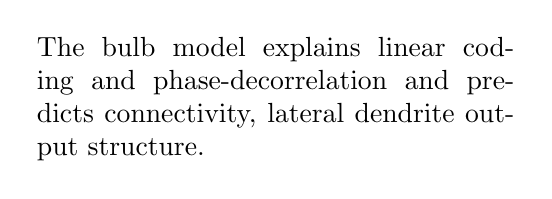
\begin{tikzpicture}
    \node[] (caption) {
        \begin{minipage}{0.5\textwidth}
            \TEXT{
                The bulb model explains linear coding and phase-decorrelation and
                predicts connectivity, lateral dendrite output structure.} 
        \end{minipage}
    };
\end{tikzpicture} \hfill%
\begin{tikzpicture}
    \node[] (result) {
        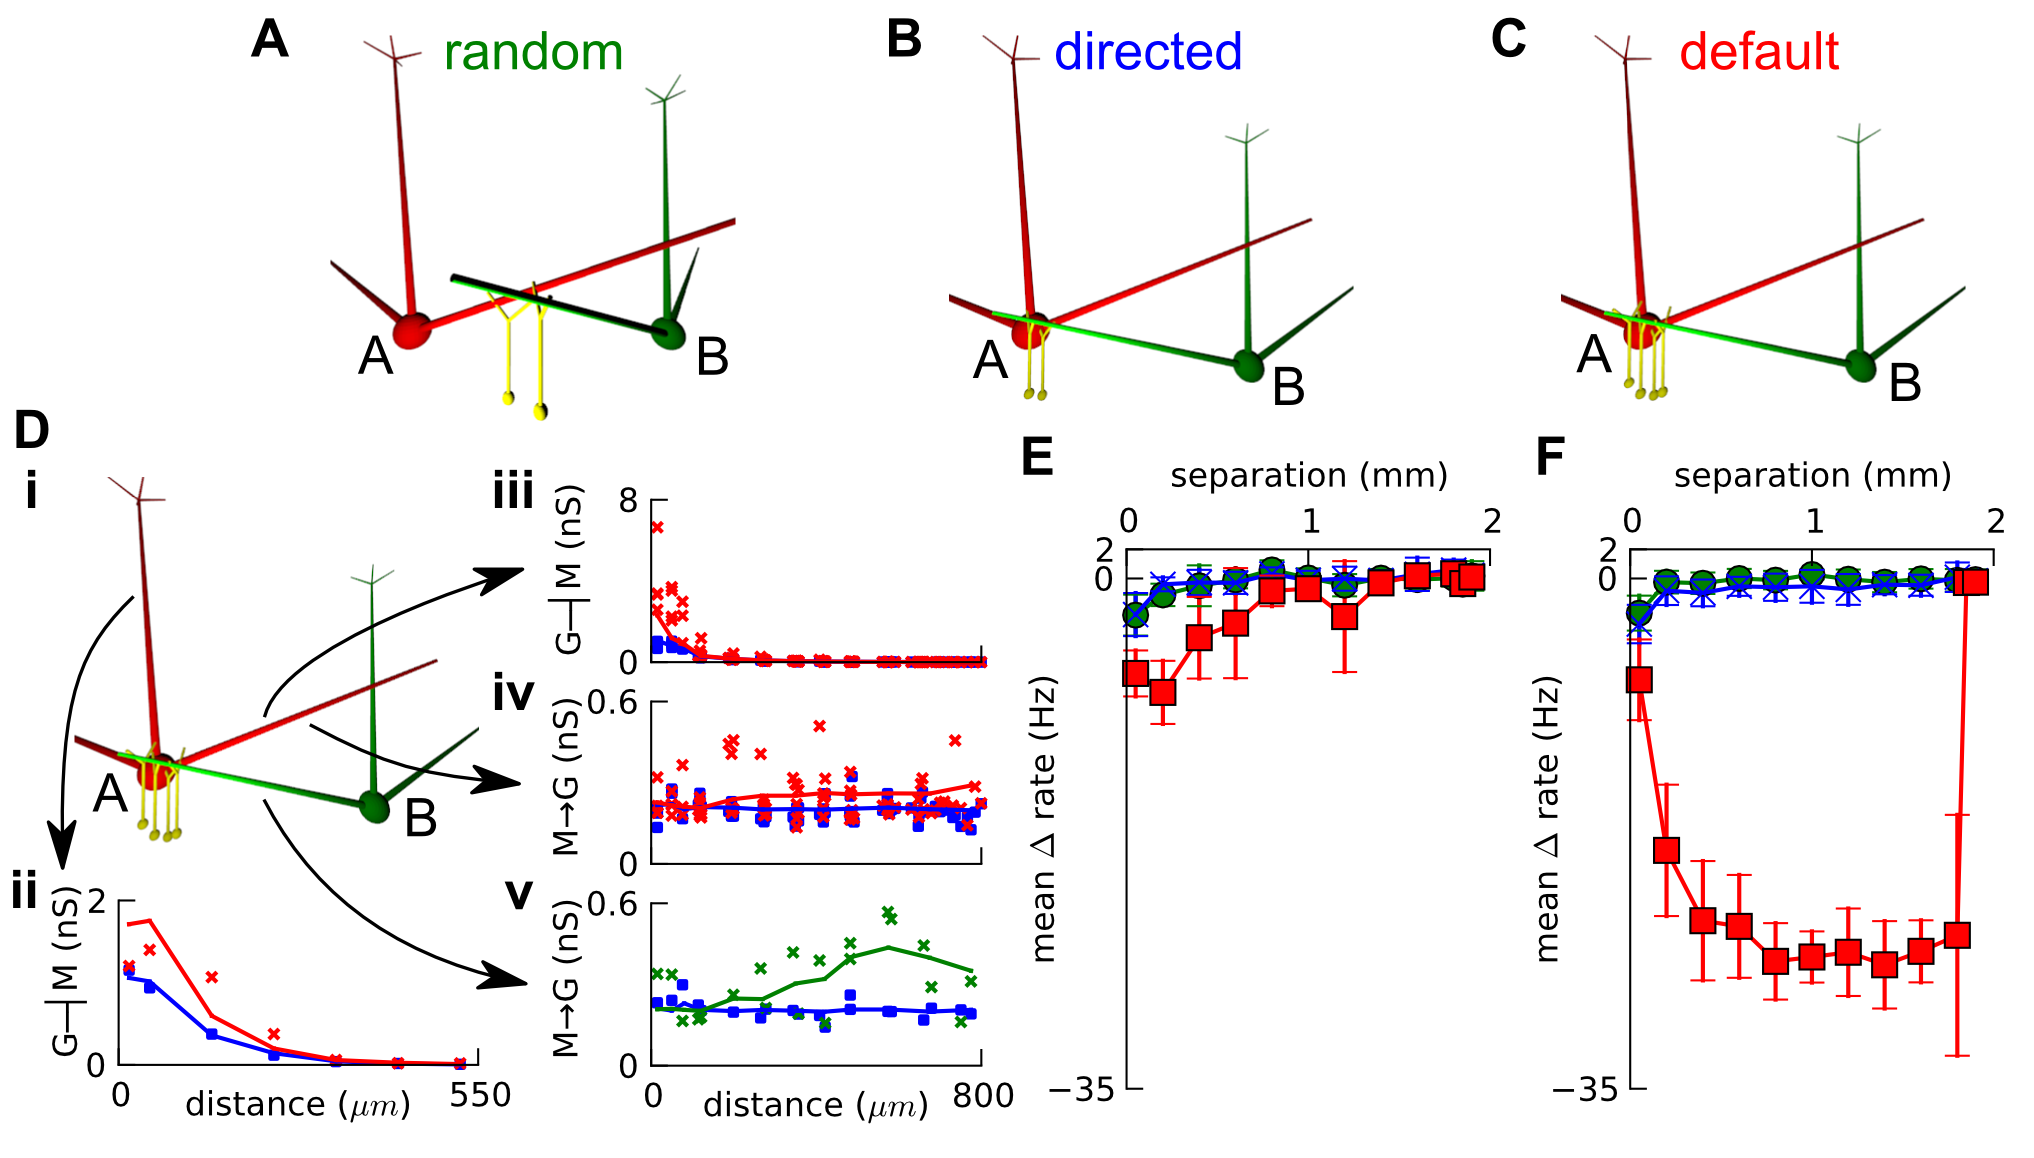
\includegraphics[width=0.45\textwidth]{./images/aditya_work.png}
    };
\end{tikzpicture}

%% One more model here.
\raggedright
\SECTION{2.3 Modelling Cortex}

\TEXT{\bf Predicts:}

\centering
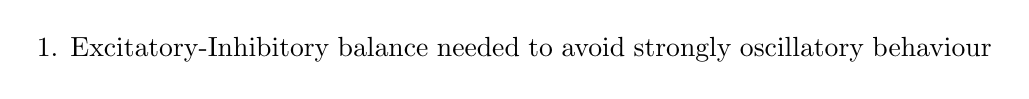
\begin{tikzpicture}
    \node [] (label) {
        \begin{minipage}{\textwidth}
            \TEXT{1. Excitatory-Inhibitory balance needed to avoid strongly oscillatory
                behaviour}
        \end{minipage}
    };
\end{tikzpicture}
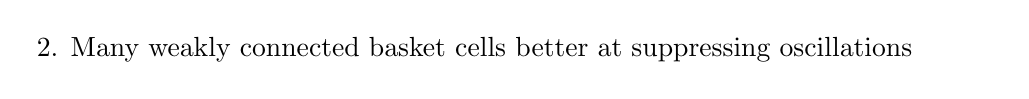
\begin{tikzpicture}
    \node [] (label) {
        \begin{minipage}{\textwidth}
            \TEXT{2. Many weakly connected basket cells better at suppressing
                oscillations}
        \end{minipage}
    };
\end{tikzpicture}

\vspace{-1cm}
\begin{tikzpicture}
    \node[] (robust) {
        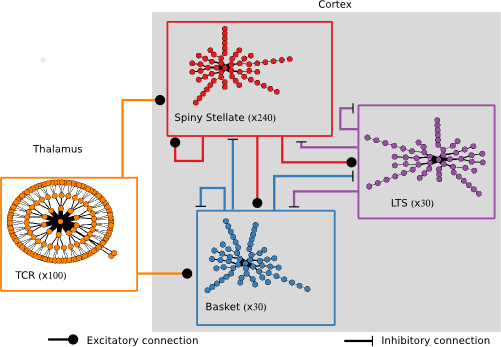
\includegraphics[width=0.9\textwidth]{./images/subha.png}
    };
\end{tikzpicture}

\end{Figure}

